
\documentclass[runningheads,a4paper]{llncs}
%\documentclass{llncs}
%

\usepackage{llncsdoc}
\usepackage{amssymb}
\usepackage{amsmath}
\usepackage[utf8x]{inputenc}

\usepackage{url}
%\usepackage{moreverb}
\usepackage{verbatim}
\usepackage{enumerate}
\usepackage{listings}
%\usepackage{fancyvrb}
%\usepackage[table]{xcolor} % to use cellcolor
\usepackage{xspace}
\usepackage{graphicx}
\usepackage{caption}
\usepackage{multirow}
\usepackage{xcolor}


\renewenvironment{description}[1][0pt]
  {\list{}{\labelwidth=0pt \leftmargin=#1
   \let\makelabel\descriptionlabel}}
  {\endlist}

\newcommand{\tth}{\texttt{ttH\_dilep}\xspace}
\newcommand{\ttDilepKinFit}{\texttt{ttDilepKinFit}\xspace}
\newcommand{\ttLoop}{\texttt{Loop}\xspace}
\newcommand{\ttDoCuts}{\texttt{DoCuts}\xspace}
\newcommand{\dilep}{\texttt{dilep}\xspace}
\newcommand{\ttbar}{$t\bar{t}$\xspace}

\begin{document}

\title{Removing Inefficiencies From Scientific Code: A Case Of The ATLAS Experiment 
\thanks{Detalhes financiamento...}}

%\end{comment}


\titlerunning{Removing Inefficiencies From Scientific Code}

% the name(s) of the author(s) follow(s) next
%
% NB: Chinese authors should write their first names(s) in front of
% their surnames. This ensures that the names appear correctly in
% the running heads and the author index.
%
\author{André Pereira\inst{1,2} \and António Onofre \inst{1,2} \and \\ Alberto Proença\inst{1}}
%
\authorrunning{Pereira, Onofre, and Proença}
% (feature abused for this document to repeat the title also on left hand pages)

% the affiliations are given next; don't give your e-mail address
% unless you accept that it will be published
\institute{Universidade do Minho, Portugal \and LIP-Minho, Portugal 
\\ \{ampereira, aproenca\}@di.uminho.pt, antonio.onofre@cern.ch}


\maketitle              % typeset the title of the contribution
%\thispagestyle{empty}
%\pagestyle{empty}

\begin{abstract}

This paper presents a set of methods and techniques for removing inefficiencies in scientific code. A scientific application, of the ATLAS experiment, is used as a case study. Here, we implement and test a set of optimizations to deal with performance inefficiencies in a organized approach: identification, removal at application development and at application runtime. These optimizations consider code, algorithm and data structure design, parallelization in shared memory systems, and runtime configurations for NUMA environments. These optimizations target different multithreading and multiprocess combinations, and CPU affinities. We expect that this communication will aid scientists to become more aware of common efficiency pitfalls in scientific code.

\keywords{High Performance Computing, Efficiency Optimization}
\end{abstract}
%

\section{Introduction}
\label{introduction}

The European Organization for Nuclear Research (CERN) is a consortium of 20 European countries, founded in 1954, with the purpose of operating the largest High Energy Physics (HEP) experiments in the world. The instrumentation used in nuclear and particle physics research is essentially divided into particle accelerators and detectors. The Large Hadron Collider (LHC) particle accelerator speeds up groups of particles close to the speed of light, in opposite directions, resulting in a controlled collision inside the detectors (each collision is considered an event). The detectors record various characteristics of the resultant particles, such as energy and momentum, which originate from complex decay processes of the collided protons. The purpose of these experiments is to test the HEP theories, such as the Standard Model, by confirming or discovering new particles and physics.

The ATLAS experiment, a key project at CERN, is conducting most of the crucial experiments on both the top quark and Higgs boson measurements. Approximately 600 millions of collisions occur every second at the LHC. Particles produced in head-on proton collisions interact with the detectors of the ATLAS experiment, generating massive amounts of raw data as electric signals. It is estimated that all the detectors combined produce 25 petabytes of data per year, and it is expected to grow after the LHC upgrade, which purpose is to increase the amount of energy of the accelerated particle beams. This data passes a set of processing and refinement until it is ready to be used to reconstruct the events by specific applications. The application varies according to the HEP theory being analysed. At this stage, different research groups in the same experiment enforce positive competition to produce quality results in a fast and consistent way.

These factors enforce the need to process more data, more accurately, and in less time. Research groups often opt to increase computational resources in a brute force approach to improve their research quality. However, applications use inefficiently the available computational resources, so, if properly optimized, the computational throughput could be highly boosted. A properly optimized application can provide an equal or greater performance increase at a much lower cost. This paper aims to provide a set of techniques to identify and remove inefficiencies in scientific applications, using a top quark and Higgs boson analysis application as a case study, to help scientist develop and optimize applications that efficiently use the available resources.

This paper is organized as follows: section \ref{problem_and_app} briefly presents the top quark and Higgs boson decay process and introduces a short characterization of the \tth application used as case study; section \ref{identification} presents and characterises the inefficiencies identified in the application; section \ref{removal} shows the process of removing the inefficiencies and optimizing the application at development and runtime stages; finally, section \ref{conclusion} concludes the paper and mentions future work.

\section{Top Quark and Higgs Decay}
\label{problem_and_app}

In the LHC, two proton beams are accelerated close to the speed of light in opposite directions, set to collide inside a specific particle detector. From this head-on collision results a chain reaction of decaying particles, and most of the final particles react with the detector allowing their characteristics to be recorded. One of the experiments being conducted at the ATLAS detector is related to the studies of Top quark and Higgs boson properties. Figure \ref{fig:ttbar} presents the schematic representation of the top quark decay (addressed as the \ttbar system).

\begin{figure}[!htp]
	\begin{center}
		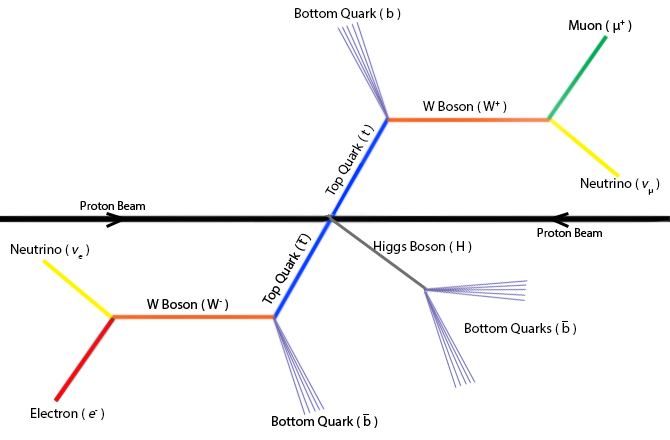
\includegraphics[scale=0.4]{images/ttbar_higgs.png}
		\caption{Schematic representation of the \ttbar system and Higgs boson decay.}
		\label{fig:ttbar}
	\end{center}
\end{figure}

The ATLAS detector can record the characteristics of the bottom quarks, detected as a jet of particles, and leptons (muon and electron). However, neutrinos do not interact with the detector and, therefore, their characteristics are not recorded. Since the Top quark reconstruction requires the neutrinos, their characteristics are analytically determined with the known information of the system, in a process known as kinematical reconstruction. The reconstruction of the whole \ttbar system has a degree of certainty associated, which determines its quality.

The amount of Bottom quark jets and leptons detected may vary between events, due to other reactions occurring alongside the Top quark decay. As represented in figure \ref{fig:ttbar}, 2 jets and 2 leptons are needed to reconstruct the \ttbar system, but the input data for an event may have many more of these particles associated. It is necessary to reconstruct the system for every combination of 2 jets and 2 leptons in the input data (referred only as combination). Then, only the most accurate reconstruction of each event is considered.

The Higgs boson is reconstructed after the \ttbar system, with the two jets that it decays to. This adds at least two more jets to the event information, increasing the number of possible combinations, as they are the same as the \ttbar system jets. The Higgs boson reconstruction uses the jets that were not needed in the \ttbar system. The overall quality of the event reconstruction depends on the quality of both \ttbar system and Higgs boson reconstructions.

The ATLAS detector experimental resolution induces an error of 2\% in each measure of the particle characteristics. The reconstruction of both \ttbar system and Higgs boson will have an error associated due to this. To improve the quality of the reconstructions it is possible to apply a random variation to the particles parameters, with a maximum magnitude of 2\%, a given amount of times and chose the reconstructions that better fits the theoretical model. The quality of the reconstructions, and application execution time, are directly proportional to the amount of variations per combination performed. The goal is to perform as many variations as possibly within a reasonable time frame.

The \tth application was designed the reconstructions of the \ttbar system and Higgs boson, as explained above. The application flow is presented in figure \ref{fig:ttbar}. The data of an event is loaded to a single global state shared among the application and the LipMiniAnalysis library, and it is overwritten every time a new event is loaded. Then the event is submitted to a series of cuts, which filter the events that are not suited for reconstruction. When an event reaches the cut 20 the \ttbar system and Higgs boson are reconstructed in a function named \ttDilepKinFit. If an event has a possible reconstruction it passes the final cut and its information is stored.

\begin{figure}[!htp]
	\begin{center}
		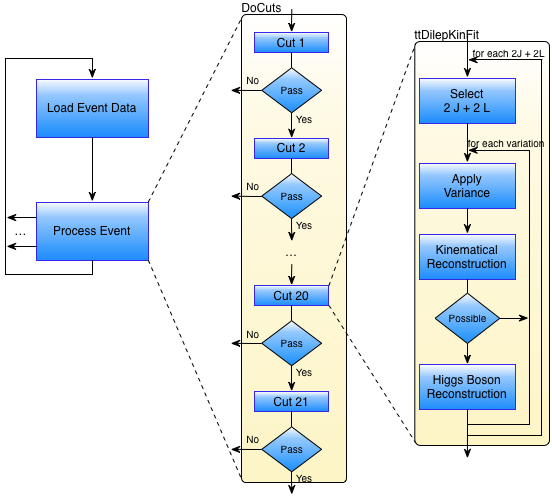
\includegraphics[scale=0.4]{images/graf_abstract_flow_with_kinfit.png}
		\caption{Schematic representation for the \tth application flow.}
		\label{fig:flow}
	\end{center}
\end{figure}

\begin{itemize}
	\item Top Quark and Higgs Boson decay from a physics point of view
	\item ATLAS detector experimental resolution
	\item ttH\_dilep brief characterisation
\end{itemize}

\section{Code an Algorithm Inefficiencies}
\label{identification}

Inefficiency removal is a two stage iterative process. First, the application is analysed to identify the critical sections of the code that take the most time to compute. This can process can be automatised by using third party tools, such as GPROF, Callgrind, or VTune, which produce reports listing the percentage of time spent in each of the application functions. A more detailed analysis can be obtained using tools similar to PAPI, where hardware counters are measured to obtain cache miss rates, float point instructions, and other low level information.

The test environment used in both this section and section \ref{removal} is a dual-socket system with two Intel E5-2670v2 with 10 cores (20 hardware threads) at 2.5 GHz each, 256 KB L2 cache per core and 25 MB shared L3 cache, coupled with 64 GB DDR3 RAM. The KBest policy was adopted to ensure that the only the best, but consistent, time measurements are considered. A 5\% interval was used for a \textit{k} of 4, with a minimum of 12 and maximum of 24 time measurements.

In a preliminary analysis using Callgrind, the \ttDilepKinFit was identified as the most time consuming function, specially when considering a significant number of variations. Figure \ref{fig:ttDilepKinFit} shows the relative execution time for the \ttDilepKinFit, I/O of event loading, and the rest of the computations (the remaining cuts). \tth execution with 1024 variations was considered for all efficiency measurements, as it is a reasonable amount without an exaggerated compromise of the application execution time. Note that the application is dependant on the ROOT framework and LipMiniAnalysis library, which code cannot be modified.

\begin{figure}[!htp]
	\begin{center}
		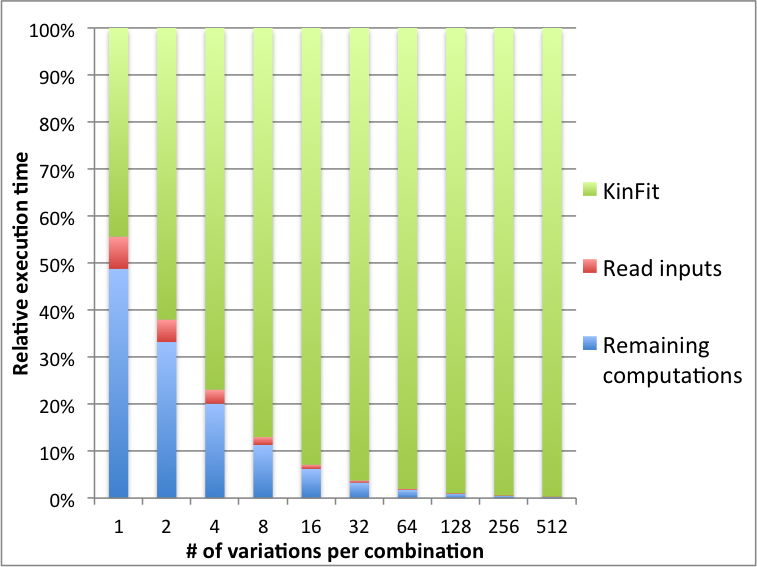
\includegraphics[scale=0.4]{charts/relative_exec_time_kinfit_rest.png}
		\caption{Relative execution time of the critical sections of the \tth application.}
		\label{fig:ttDilepKinFit}
	\end{center}
\end{figure}

A preliminary computational analysis determined that the application is compute bound on the test system, where accesses to the system RAM memory are not a limiting factor with a ratio of 8 instructions per byte fetched for 512 variations.

\subsection{Pseudo-Random Number Generation Inefficiencies}

Pseudo-random number generators (PRNGs) are common in many Monte Carlo simulation and reconstruction applications. A good PRNG deterministically generates uniform numbers with a long period, its values produced pass a set of randomness tests, and, in HPC, it must be efficient and scalable. Repeatability is ensured by providing a seed to the PRNG prior to number generation, due to their deterministic execution.

The variation for the kinematical and Higgs reconstructions is based on applying a random offset to the current particles characteristics. This offset has a maximum magnitude of 2\% of the original value and is determined by a PRNG. An analysis of the callgraph produced for 256 variations (higher variations made the Callgrind execution time infeasible) revealed that 63\% of \tth execution time was spent on the PRNG. However, 23\% of the time was spent on setting the seed for the PRNG. Figure \ref{fig:prng256} presents the callgraph for the \ttDilepKinFit function of \tth.

\begin{figure}[!htp]
	\begin{center}
		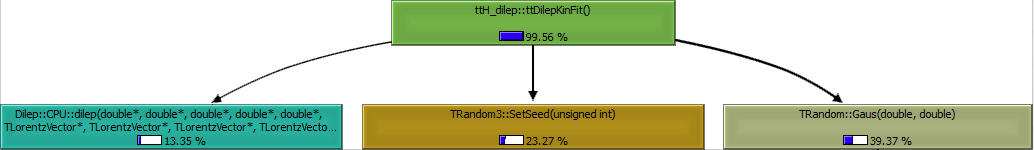
\includegraphics[scale=0.33]{images/prng_256.png}
		\caption{Callgraph subset of the \ttDilepKinFit most time consuming sections for 256 variations per combination.}
		\label{fig:prng256}
	\end{center}
\end{figure}

An analysis of the code revealed that the application uses a PRNG available in ROOT, which uses the Mersenne Twister algorithm, resetting the seed in every variation. The Mersenne Twister period is approximately $4.3 * 10^{6001}$, while the maximum amount of pseudo random numbers generated by the application, for the input file used and 512 variations, is $1.5 * 10^9$, making the seed reset unnecessary. The removal of this inefficiency granted an increase of 71\% in performance for 1024 variations.

%\begin{figure}[!htp]
%	\begin{center}
%		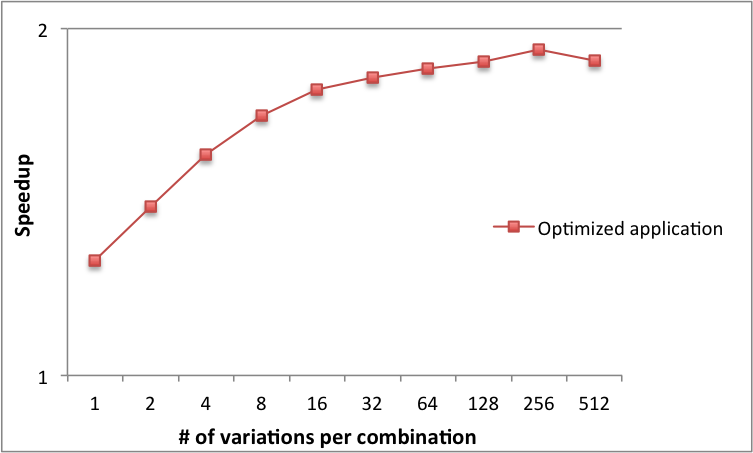
\includegraphics[scale=0.4]{charts/speedup_trandom_optim.png}
%		\caption{Schematic representation for the \tth application flow.}
%		\label{fig:PRNG}
%	\end{center}
%\end{figure}

\subsection{Data Structure Inefficiencies}
\label{data_inef}

Even with the PRNG optimization the \ttDilepKinFit remains the critical region in the application. An analysis of the functions code revealed that there are no relevant code inefficiencies left, so the next step is to parallelize \ttDilepKinFit. Note that it is not possible to parallelize the whole event processing since only one is loaded at a time and part of its information is stored in LipMiniAnalysis library, which we did not have permission to refactor. Besides not allowing this parallelization, reading events individually is more inefficient than reading all events at once, where in the former slower random reads are made on the hard drive and in the latter the fast sequential reads are used.

\subsubsection*{Optimization Approaches}

Parallelizing \ttDilepKinFit implies modifying its flow. Currently, the data of each variation is overwritten when processing each different combination of an event, so a data structure holding all combinations of the event is necessary. Picking a lepton/jet combination depends on all previous combinations chosen, which serializes the construction of the data structure. Each parallel task (indivisible work segment) selects a combination with variations still to compute, then varies the particles parameters, performs the kinematical reconstruction, and attempts to reconstruct the Higgs boson. A parallel merge is performed after all combinations are computed to get the most accurate reconstruction for the event. Figure \ref{fig:SeqPipeline} presents the sequential and parallel workflow for \ttDilepKinFit.

\begin{figure}[!htp]
	\begin{center}
		\raisebox{-0.5\height}{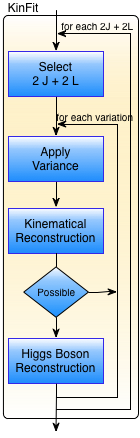
\includegraphics[scale=0.5]{images/sequential_kinfit.png}}
		\raisebox{-0.5\height}{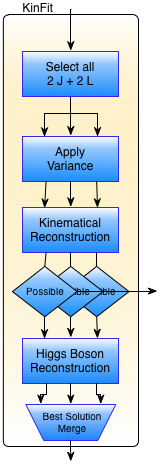
\includegraphics[scale=0.5]{images/parallel_kinfit.png}}
		\caption{Schematic representation of the \ttDilepKinFit sequential (left) and parallel (right) workflows.}
		\label{fig:SeqPipeline}
	\end{center}
\end{figure}

A shared memory parallelization using OpenMP was devised, as it is the bes approach for single shared memory systems. The parallel tasks are grouped into threads, which holds the best reconstruction to minimize the complexity of the merge by reducing through all the threads instead of tasks. The amount of tasks for each thread is balanced dynamically by the OpenMP scheduler, as the workload is irregular since the Higgs boson reconstruction execution is not always computed. Each thread has a private PRNG initialized with different seeds to avoid correlation between the numbers generated.

\begin{figure}[!htp]
	\begin{center}
		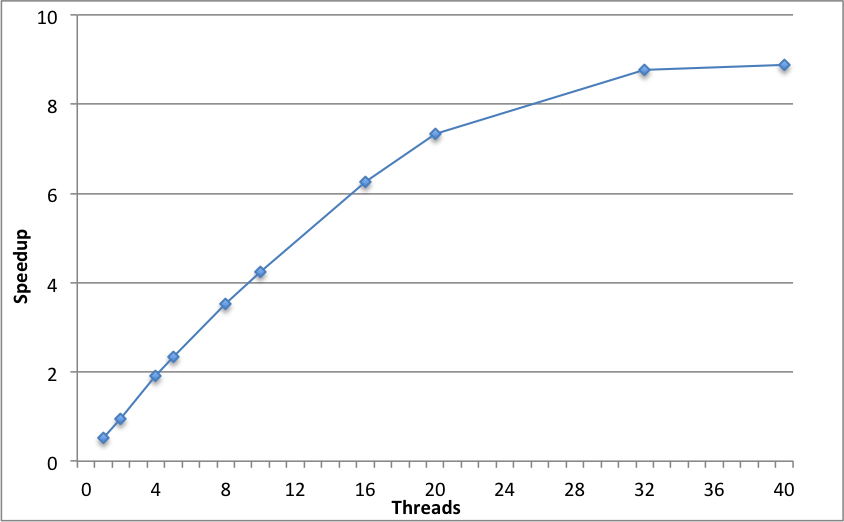
\includegraphics[scale=0.4]{charts/speedup_non_pointer_omp.png}
		\caption{Speedup for \tth parallel non-pointer version application.}
		\label{fig:non_pointer_speedup}
	\end{center}
\end{figure}

Figure \ref{fig:non_pointer_speedup} presents the speedups for various variations and threads. The purpose of the 1 thread test is to evaluate the parallelization overhead. The application has a constant scaling up to 64 variations but tends to stabilize for more variations. The best efficiency occurs when using 2 and 4 threads, where the application is almost using all resources from the cores used. The best overall performance occurs for 40 threads, but it only offers a speedup of 8.8, underusing the available 20 physical cores. Note that there is no significant overhead due to NUMA accesses, as seen by the constant increase in performance from 10 to 16 threads.

% ------------- pointer version abaixo -----------------

The lack of performance means that there are still inefficiencies on the application, probably caused by the parallelization overhead. Intel's VTune was used to search for hotspots (bottlenecks) on the parallel \tth, since this tool is best suited for profiling parallel applications while providing an easy to use GUI. A preliminary analysis revealed that the application was spending around 20\% of the time building the combination data structure for 256 variations.

An analysis of the data structure code revealed that there were inefficiencies that were affecting the performance in specific situations. Data that is read-only on the parallel section is being replicated in each element of the data structure. If the elements were to share a pointer to such data, the overhead of constructing the data structure would be reduced. However, this could lead to worse cache management, due to cache line invalidations proportional to the number of threads, resulting in added overhead, specifically in NUMA environments where the communication cost is increased. Nevertheless, this optimization was implemented and tested (addressed as \textit{pointer version}), with its speedups presented in figure \ref{fig:pointer_speedup}.

\begin{figure}[!htp]
	\begin{center}
		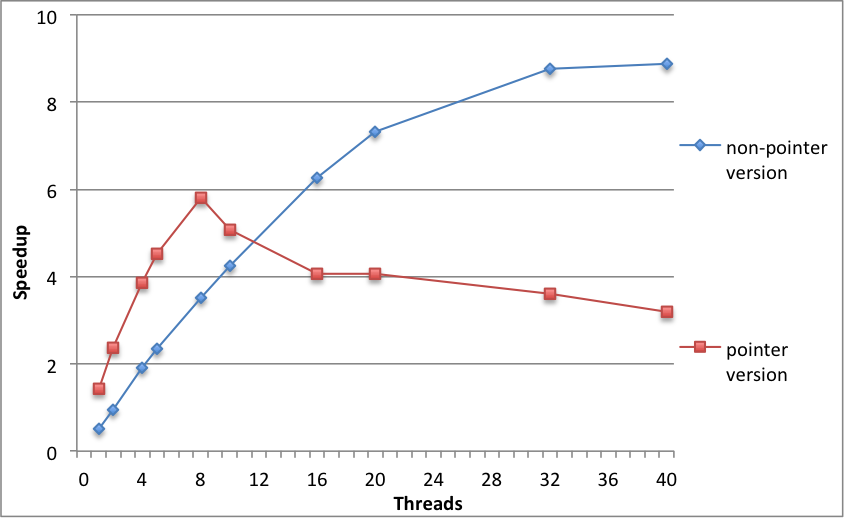
\includegraphics[scale=0.4]{charts/speedup_pointer_omp.png}
		\caption{Speedup for \tth parallel pointer version application.}
		\label{fig:pointer_speedup}
	\end{center}
\end{figure}

As predicted, the best speedup occurs when using only one CPU device, specifically for 8 threads. Even with 10 threads the performance of the application suffers due to the increase of concurrent accesses to the L3 cache on the system due to the shared data. This decrease in performance is even more noticeable when using both CPU devices, where the non-pointer version still scales while this version performance is worse than with one CPU device. However, this implementation is more efficient than the former when using only one device. Note that the superlinear speedups is due to the reduction in the data that each thread has to process, making it suitable to be stored in the private L2 cache of each core, avoiding the slower accesses to L3 cache.

\section{Runtime Inefficiencies}
\label{removal}

When submitting a job or application for execution on a given computing system, most users trust the default configurations of the submission environment. However, if the user needs to improve the efficiency of the code execution, he/she must be aware of the environment variables that can be controlled and how those can impair the performance. Two cases will be addressed here: (i) how to spread the code parallelism, between processes and threads, and (ii) how to allocate the available cores on each device to threads and processes.

\subsection{Multithreading Inefficiencies}

Without the sensibility provided by the tests in section \ref{identification}, a scientist would incur in the pitfall of using all available cores on the system (and even all hardware threads, if each core supports hardware multithreading), hoping that it would provide the best performance. While it may be true for the non-pointer implementation, the system computational resources would be inefficiently used, and using the single device highly efficient pointer implementation would induce a even greater waste.

A closer look to the pointer based implementation shows in fact that it is the most efficient one. As seen in section \ref{data_inef}, the scalability of the parallelization is limited by the NUMA organization on modern multiple CPU device systems. If the threads on $cpu_1$ do not share information with the threads on $cpu_2$, the NUMA bottleneck is removed by using multithreaded processes. However, parallelization at the process level, where each process performs a data analysis on a separate event, is not possible with the current implementation of LipMiniAnalysis, where a single global state is allocated to store data from each event processing.

Data analysis applications are individually executed for each file (around 1GB in size) in a very large set of files, at a terabyte scale, received weekly from CERN. An alternative approach to the process parallelization over a single input data file is to balance the execution of different \tth processes in the system on a set of distinct input files. This reduces the complexity of the implementation, with no changes needed for \tth, and avoids communication between processes. A simple scheduler was devised, which takes a set of input files and spawns a given amount of \tth processes. The scheduler dispatches the files to the different processes in a queue-like approach, and monitor their execution as shown in figure \ref{fig:sched_flow}. A set of 20 input files was considered for testing and evaluation purposes, with different configurations of processes and threads per process.

\begin{figure}[!htp]
	\begin{center}
		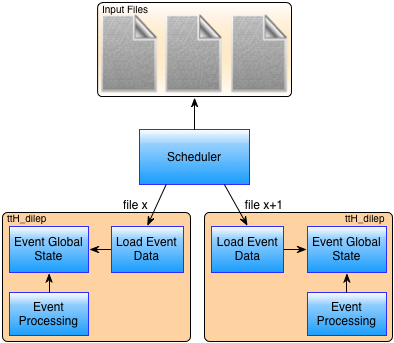
\includegraphics[scale=0.5]{images/scheduler_workflow.png}
		\caption{Schematic representation of dispatcher workflow.}
		\label{fig:sched_flow}
	\end{center}
\end{figure}

Figure \ref{fig:Sched} presents the speedups using 2, 4, 5, 8, and 10 processes for various thread configurations, with maximum number of threads limited to 40. A higher amount of processes was not tested as the efficiency decayed from 8 to 10 processes. The best speedups occur for 8 processes with 5 threads each, with a peak of 69.3, 7.8 and 11.7 times better than the best non-pointer and pointer implementations, respectively. A small number of threads such as this allows for a small overhead in the \tth parallelization, namely on load balancing and final best reconstruction merge for each event. For 10 processes the load on the system due to the lack of shared memory and I/O operations affects the performance, decreasing the speedups relatively to using 8 processes. A common behaviour is that when using the CPU devices hardware multithreading the speedups tend to stabilize, or even drop in the case of 2, 4, and 5 processes.

\begin{figure}[!htp]
	\begin{center}
		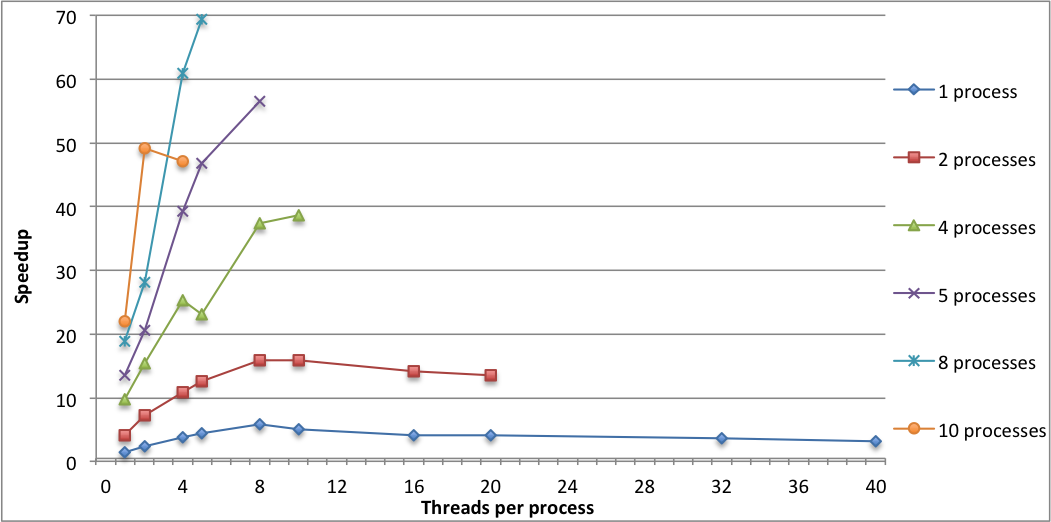
\includegraphics[scale=0.5]{charts/speedup_sched.png}
		\caption{Speedups for the scheduler with the pointer based implementation for 2, 4, 5, 8, and 10 processes and various threads per process.}
		\label{fig:Sched}
	\end{center}
\end{figure}

\subsection{Core Affinity Inefficiencies}

The key issue in runtime efficiency is the thread affinity, namely to, control the allocation of each thread to which CPU core. By default, OpenMP lets the operating system to manage the thread affinity; as consequence, threads may migrate among cores during runtime. If a thread is running on core $c_1$ and moves to core $c_2$, all data on the private cache $l_{c_1}$ needs to be reloaded to cache $l_{c_2}$, causing unnecessary overhead. This effect is amplified if the threads are moved between adjacent CPU devices. When multiple different, and (possibly) parallel processes are running on the same system, which is common in production environments, such scheduling occurrences happen more often.

Defining the thread affinity of an application may provide a more predictable, or in some cases better, performance. In theory, an optimum thread affinity scheme allocates the threads to contiguous physical cores of one CPU device, uses the cores of the second CPU device only after the first is filled, and finally uses the multithreading after filling all physical cores. Note that using multithreading before the second CPU device is fully occupied may provide better performance in memory bound applications. This type of affinity must be defined prior to the application execution and depends on the system used. In this data analysis case the affinity was specifically tuned to this 20-core system for all threads or process/threads configurations for the scheduler.

\begin{figure}[!htp]
	\begin{center}
		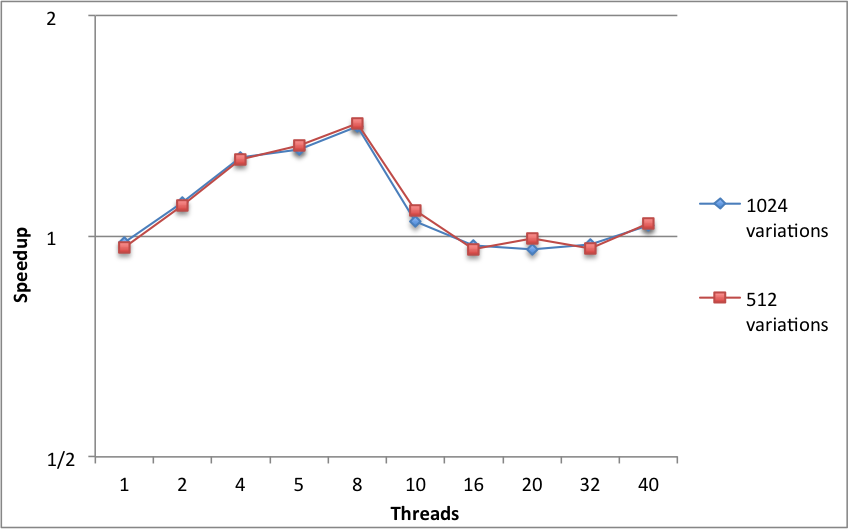
\includegraphics[scale=0.55]{charts/speedup_pointer_aff.png}
		\caption{Speedup of the \tth parallel pointer implementation with core affinity.}
		\label{fig:pointer_aff}
	\end{center}
\end{figure}

By analysing the speedups of the pointer implementation of \tth with thread affinity, in figure \ref{fig:pointer_aff}, the specification of the affinity provides speedups for the previous most efficient number of threads, i.e., up to 8 threads. For 8 threads the performance increases by 41\%, relative to its no affinity counterpart. With this number of threads, and the amount of shared data, moving threads between cores at runtime causes more cache warm ups to occur, significantly affecting the performance. When using more than 10 threads the application is roughly 4\% slower as the operating system uses some multithreaded cores rather than using all available physical cores and it does a better job at managing the multithreading.

The same affinity study was performed on the scheduler for 512 and 1024 variations per combination, with their speedups presented in figure \ref{fig:sched_aff}. For 1024 variations the performance is increased for specific configurations, only diminishing the performance of 5 processes, peaking at 52\%, 90\%, 8\%, and 25\% for 2, 4, 8, and 10 processes respectively. For 512 variations the improvement is more constant but smaller, peaking at 72\%, 28\%, 37\%, 11\%, and 5\% for 2, 4, 5, 8, and 10 processes respectively. There are only few cases that the performance is worse.

\begin{figure}[!htp]
	\begin{center}
		\raisebox{-0.5\height}{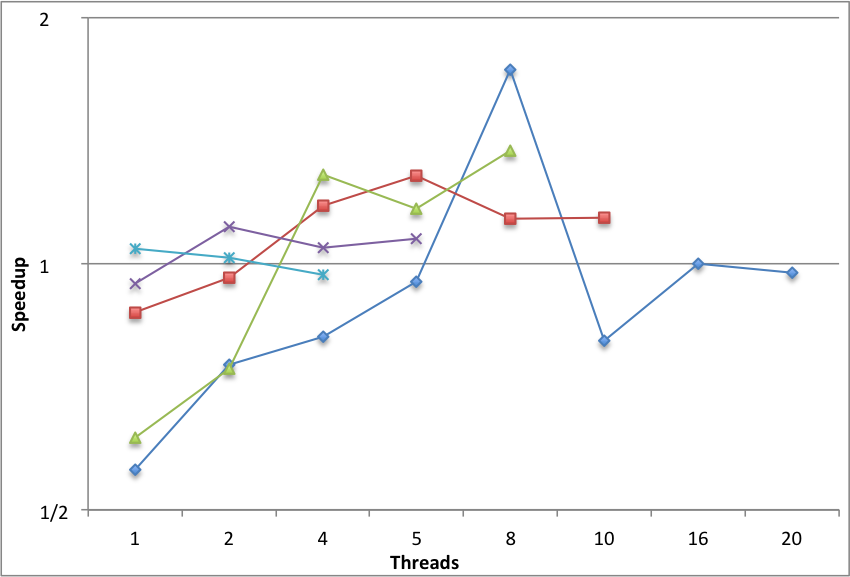
\includegraphics[scale=0.378]{charts/speedup_sched_aff_512.png}}
		\raisebox{-0.5\height}{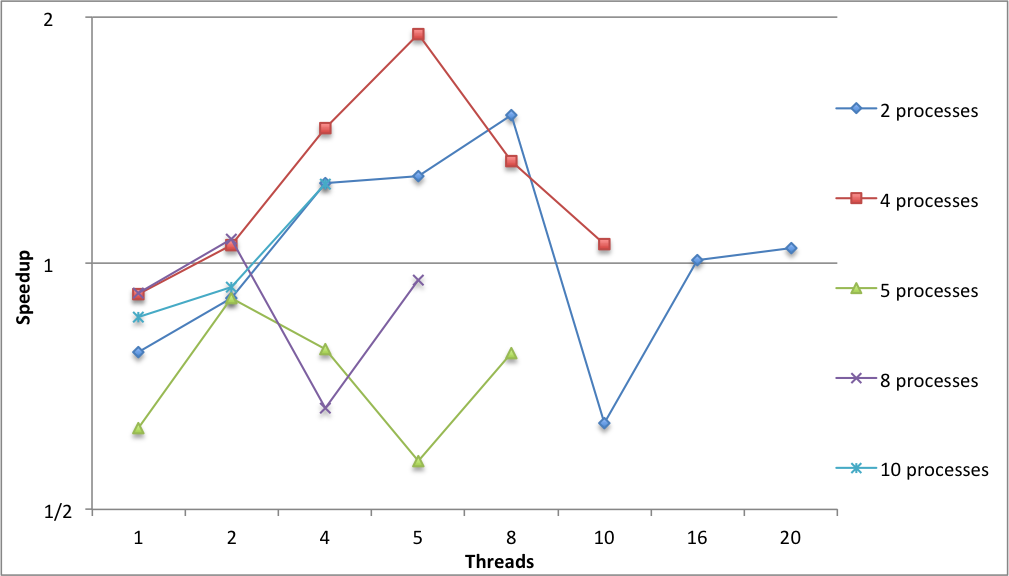
\includegraphics[scale=0.378]{charts/speedup_sched_aff_1024.png}}
		\caption{Speedups of the scheduler with the pointer based implementation for 512 (left) and 1024 (right) variations and various threads per process with core affinity.}
		\label{fig:sched_aff}
	\end{center}
\end{figure}

The performance with core affinity is less susceptible to oscillations, as with no affinity it is sometimes affected by OS thread reallocations. It is when the reallocations occur that setting the core affinity provides the best performance. Otherwise it does not allow to use multithreading (unless it is in the scheme) for hiding the memory accesses latency, affecting the performance. For 512 variations, the applications execution time is smaller meaning that the impact from thread reallocations is higher, benefiting from setting the core affinity. It is not possible to use a theoretical affinity scheme for always improving the performance on every system, as it is highly dependent on:

\begin{itemize}
	\item The algorithm, as memory bound algorithms suffer more from core reallocation due to the losing all data on cache, where fixing their position on a specific core avoids unnecessary accesses to the RAM;
	\item The application execution time, as the impact from thread reallocations is higher in faster applications;
	\item The operating system, as OpenMP, by default, lets it manage the thread allocation and it is susceptible to the overall system load, causing fluctuations in consecutive applications execution time.
\end{itemize}

With all optimizations considered, the best overall performance in a dual 10-core Xeon system is obtained using the scheduler combined with the pointer implementation, with 8 multithreaded processes (with 5 threads each), reaching a speedup of 113 over the original sequential application.

\section{Conclusion}
\label{conclusion}

This paper presents a study of the inefficiencies in scientific code, using a particle reconstruction analysis application as a case study. Top quark and Higgs boson studies require reconstructing from measurements of a very large number of particle collisions, performed weekly by the \tth application on terabytes of data. A faster and more accurate analysis of the data allows to better reconstruct more particle collisions and to improve the quality of the research results.

We identified and removed inefficiencies in different stages of the application: when designing the code, and during its submission for execution. In the code design, inefficiencies in the pseudo-random number generation were tackled, a common component of most simulation and analysis applications, which led to 71\% performance improvement. In data structure design, by analysing the factors limiting the particle reconstruction parallelization, and presenting and testing two alternative solutions for shared memory environments. The non-pointer implementation had a constant scaling on a dual-socket NUMA system, while the pointer implementation was much more efficient using a single CPU.

At application runtime, a multiprocess approach using the more efficient parallel implementation tackled its inefficiencies on NUMA systems, providing a maximum speedup of 69.3. An efficient control on the thread affinity of this implementation provided a performance improvement up to 90\%. However, the fluctuation in performance and the dependencies on many system characteristics prevented the definition f a generalized heuristic to aid to control the best affinity for the application, for any computing system.

\begin{figure}[!htp]
	\begin{center}
		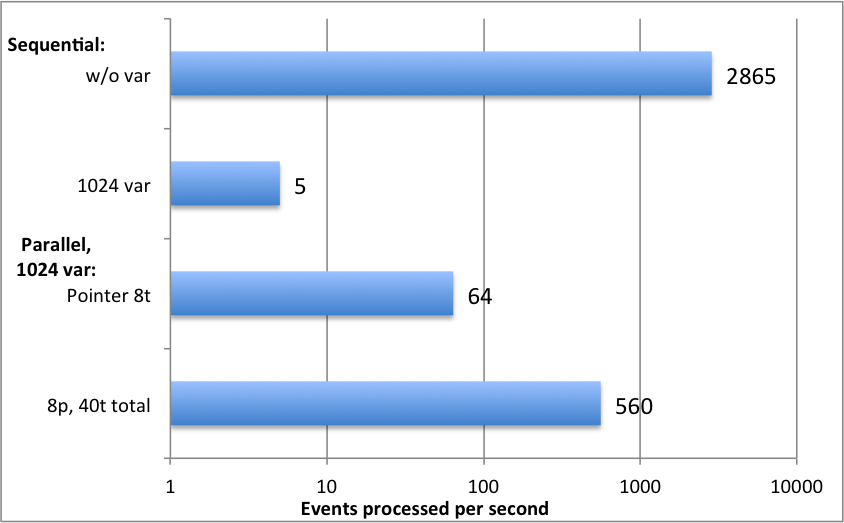
\includegraphics[scale=0.55]{charts/events_per_sec.png}
		\caption{Throughput of events processed for the original sequential \tth,with no and 1024 variations (\textit{var}), and for the parallel pointer and multiprocess implementations (with \textit{t} being threads and \textit{p} processes).}
		\label{fig:events_sec}
	\end{center}
\end{figure}

Figure \ref{fig:events_sec} plots the number of events processed per second in the original sequential application without variations of the particle characteristics, for 1024 variations, and for the parallel pointer and multiprocess implementations for 1024 variations. Using a single process, the throughput improves by a factor of 12.8, from 5 to 64 events per second, using a single CPU device. The best overall performance, for the multiprocess implementation with 8 processes with 5 threads each, provided an improvement by a factor of 113 on event throughput, from 5 to 560 events per second.

There are other important aspects that improve code efficiency, which were not taken into consideration. The compiler, and respective optimization options, can have a big impact in application performance, where different options may be best suited for certain applications than others. Rules for writing vectorized code were not presented but may improve the efficiency when processing large amounts of data, as the compiler is not able to perform most code modifications necessary to take advantage of vector instructions. Using efficient numeric libraries\cite{MKL,BLAS} when required usually has a big impact on performance. There are guides that provide rules and present techniques for developing efficient code\cite{Intel:Optimization,Intel:DevOptimization,NUMA}.

We hope to improve the sensibility of scientists to the efficiency pitfalls common in scientific code, to help develop more efficient and performing applications. The performance of the \tth application was improved by a factor of 113, for the test system used, helping physicists to execute more particle collisions with a more refined reconstruction process, which efficiently uses the available computational resources.

Even with the interesting improvements to the application efficiency, some directions of future research were identified. The scheduler could be improved to automatically predict the best process/thread configuration for each system by analysing a set of micro-benchmarks or the application itself on a small input, and ultimately identify the best core affinity scheme. Also, the application efficiency could be improved using hardware accelerators, balancing the workload among accelerators and CPU devices in heterogeneous systems. Frameworks for parallelization and workload balancing for heterogeneous systems can be analysed and tested with this case study.


% Acknowledgements

\paragraph{Acknowledgments:}


\bibliographystyle{splncs}
\bibliography{my}


\end{document}
